\section{Introductory thoughts}
To start, a small introduction to ADflow's solvers, its history and the initial
state of SST is given.

In the beginning, this solver was called \textit{Standford University
Multiblock (sumb)}. It was intended as a multiblock solver for turbomachinery.
Later on, it was extended to be used in optimizations. For this, an adjoint
solver was needed. As explained in section \ref{sec:gradient_computation}, the
adjoint method needs partial derivatives which are obtained through means of
finite differences and/or automatic differentiation. For the AD part, a tool
called \textit{tapenade}
\footnote{\url{http://www-tapenade.inria.fr:8080/tapenade/index.jsp}} is used.
It automatically differentiates FORTRAN source code. But to get it working, a
lot of the initial structure had to be changed.




\subsection{Flow Solvers}
\label{sec:flow_solvers}
ADflow has three different solvers available to solve the RANS equations:
\textit{multigrid (MG)}, \textit{Newton-Krylov (NK)} and \textit{Approximate
Newton-Krylov (ANK)}. It is possible to switch between
the different solvers during a solution run. This allows to use each Solver
when it is most efficient: initiate the simulation using multigrid, once a
certain level of convergence is reached, engage the ANK solver an finally
converge the last couple order of magnitudes using the NK Solver.
\footnote{Please note that the ANK solver by itself is sufficient as a startup
strategy and MG is not necessarily needed.}

Multigrid is the baseline solver that was implemented first. It uses either the
Runge-Kutta (RK), or the Diagonalized Diagonally-Dominant Alternating Direction
Implicit (D3ADI) algorithm as a smoother. The turbulence model is solved in a
decoupled manner and using the Diagonalized Alternating Direction Implicit
(DADI) method.

The Newton-Krylov solver solves the nonlinear system of governing equations by
simply using the Newton's method. To solve this linear system, the GMRES
algorithm is used. The turbulence variables are solved in a coupled manner and
thus no other solvers are needed. This method is equivalent to using Euler's
method with an infinite time step. It is most efficient when the solution is
already at the final stages of convergence. If it is used in the early stages,
it most likely stalls.

The Approximate Newton-Krylov is similar to the NK solver in that it also uses
Euler's method. But its time step is adjustable. At the beginning of the run,
it is quite low and thus increases the stability. This allows it to be used
as a startup strategy where the NK solver wouls most certainly fail. The
lower the residual norm is, the more the time step is increased. And as such, it
approaches Newtons' method. It is subdivided into three different sub-solvers:
\textit{First order ANK (ANK)}, \textit{Second Order ANK (SANK)} and
\textit{Coupled ANK (CANK)}. Please note, the combination of both
\textit{Coupled Second-Order ANK (CSANK)} is also possible.

In its base configuration (ANK) uses a first-order routine for the residual
Jacobian and thus only affects convergence, but not the solution accuracy. Once
a user defined level of convergence is reached, the solver switches to an exact
Jacobian formulation (SANK). In these two stages, the turbulence model is
solved in a decoupled manner. Once can choose between a second
turbulence-only-ANK solver or the above mentioned DADI method. It is done this
way because the turbulence models in RANS simulations are notoriously difficult
to converge. Once again, when the residual norm reaches a user-defined level,
the coupled mode is enganged. In that state, only one ANK solver remains which
solve the flow and turbulence variables simultaneously. This helps to improve
the convergence in the later stages. \cite{adflow_solvers}




\subsection{Adjoint Solver and total derivatives}
When computing the total derivatives, it is important to realize that the
adjoint solver is not the whole story. Take a look at figure \ref{fig:MACH}. It
shows the flow of data for a simple airfoil optimization example.

\begin{figure}[H] \centering
    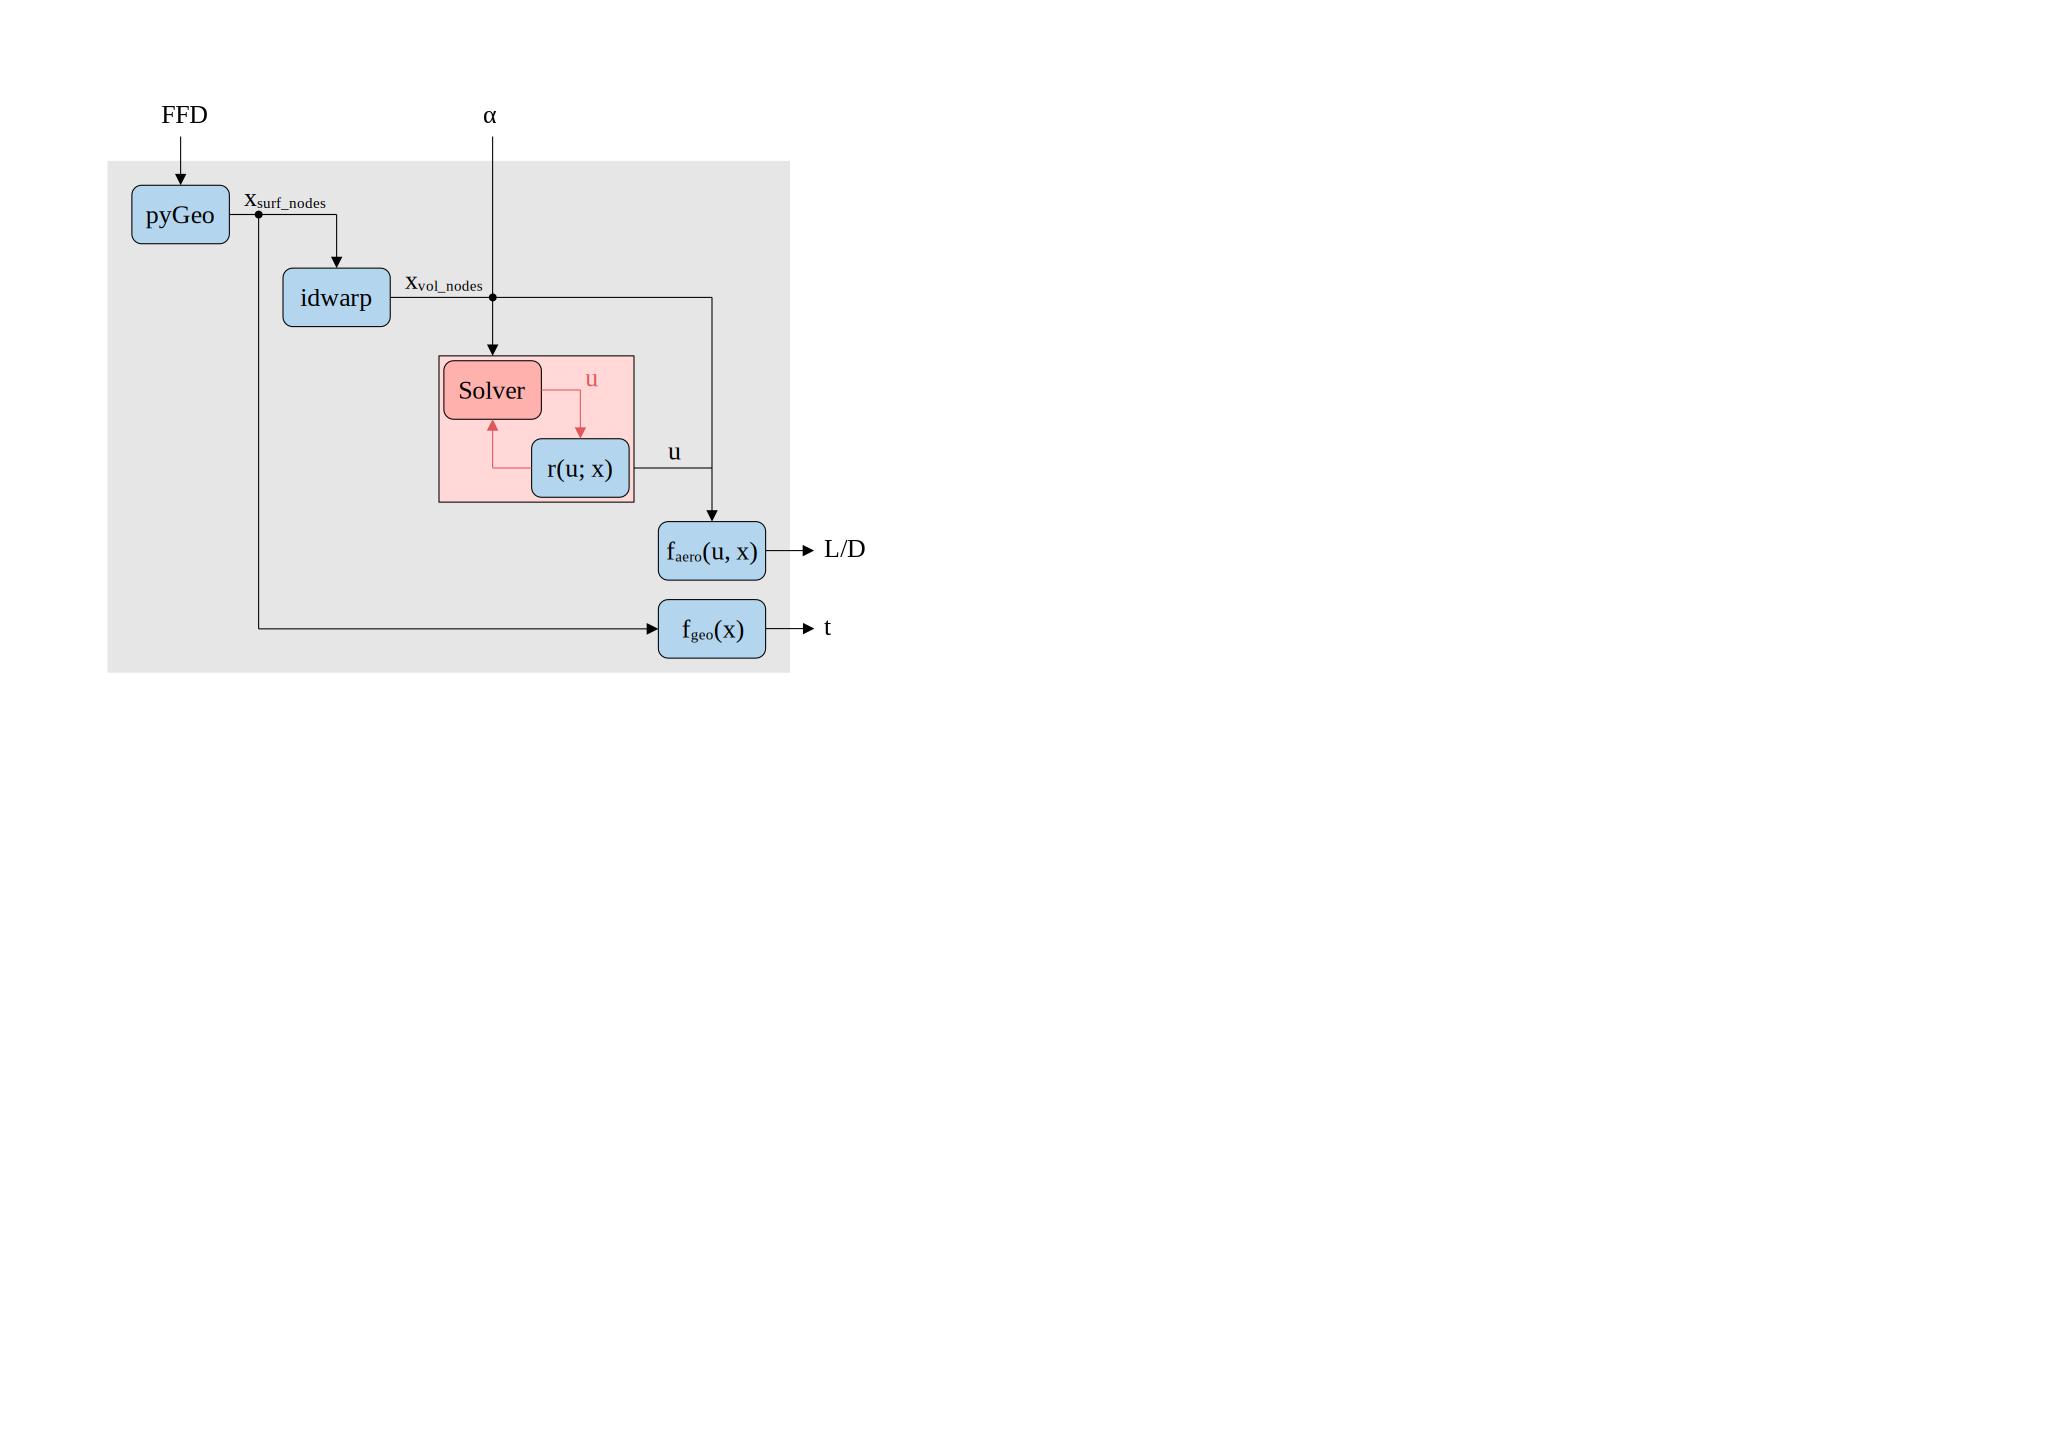
\includegraphics[width=0.7\textwidth]{MACH}
    \caption{Gradient computation dataflow in the MACH-framework. \cite{cm1}}
    \label{fig:MACH}
\end{figure}

\noindent The design variables flow in from the top. In this case it is the
angle of attack and the FFD-box that parametrizes the airfoil geometry. The FFD
DVs flow into a package called \textit{pyGeo}, it defines the connection
between the FFD points and the surface mesh. These points are then pushed into
\textit{idwarp} which deforms the volume mesh. The mesh and the aerodynamic
design variables (angle of attack in that case) is feed into ADflow. There, the
adjoint solver (red box) solves the adjoint system. Then, the solution solution
(e.g. pressure) is integrated to obtain the aerodynamic functions of interest
(in this case L/D). Please note that the geometric functions of interest (here
it is the airfoil's area) do not depend on the flow solution and thus bypass
the adjoint system. 

This has been a short summary of what is going on, the interested reader my
learn more about it in \cite{cm1}.




\subsection{Initial state of SST}
When sumb was developed initially, a multitude of different turbulence models
were implemented such as Spalart-Allmaras (SA) or SST. When the code was
overhauled for optimization, only the SA model was carried over and
differentiated. At that point SST would throw NaNs\footnote{Not a Number} and
crash. Lately, this was fixed to a point where the DADI turbulence solver would
work \footnote{See pull request:
\url{https://github.com/mdolab/adflow/pull/107}}. To summarize, before this
project started, the code for SST was there and could be solved using ANK/SANK
and the decoupled DADI turbulence solver. But nothing was differentiated which
means, the adjoint, NK and coupled ANK solvers were not usable.








\section{Needed changes}
ADflow can parallelize the computation over multiple cpus and computers. It
does this by splitting up the computational domain into blocks. These blocks
may live on different cpus or computers. As those blocks do not live in
isolation and do depended on each other, adjacent blocks need to exchange
information. ADflow uses the \textit{halo cell} approach for this. The idea is
to have imaginary ghost (halo) cells around each block. Then they are filled
with the values from the adjacent blocks. Figure \ref{fig:halo_cells} shows
this idea. ADflow can employ second order discretizations and thus needs two
layers of halo cells.

\begin{figure}[H] \centering
\includegraphics[width=0.7\textwidth]{halo_cells}
    \caption{A block split in 4 (left) and its corresponding halo cells (right)
            \cite{cfd_halo}.}
    \label{fig:halo_cells}
\end{figure}




\subsection{Halo exchange and AD}
This halo exchange is straight forward when one does not care about automatic
differentiation. But we do, and as such, some things need to be considered. The
exchanges is performed using the \textit{Message Passing Interface (MPI)}.
Unfortunately, tapenade can not handle MPI calls. To make this work, the
differentiated code is divided into parts: The \textbf{math heavy} part is
differentiated using tapenade. The \textbf{remaining part} is
hand-differentiated. This is not a big problem as this part mostly consists of
calling the AD part and performing communication. 

The turbulence model is considered a math heavy part that is automatically
differentiated using tapenade. For SA, this was straight forward as there is no
communication going on. But SST has one special case: The blending function
$\mathbf{F_1}$ (equation \ref{eq:f1}). The problem is, it is not a normal
turbulence working variable (such as $k$ or $\omega$) and thus is not exchanged
using existing infrastructure. The developers of sumb fixed this by exchanging
it manually after computing it. This is done in the model itself and was no
problem because nobody intended to AD it. \\

Now the question is: Why was it done this way and how do we get rid of this
intermediate communication?

The first part of the questions might be explained by fact that sumb was
initially developed in the early 2000's. Back then, computing power was more
expensive and computing the same $F_1$ value on different blocks was
wasteful. The cost of communication was negligible in comparison. This did not
really change, but computing power became a lot cheaper. So if it makes AD
easier, it is a good trade to get rid of the communication.








\section{Changes to wall distance}
We settled on the idea of computing $F_1$ in the halo cells instead of
communicating it across. To do this, we need to take a closer look at $F_1$. It
depends on $arg_1$ (eq. \ref{eq:arg1}) which also depends on $CD_{kw}$ (eq.
\ref{eq:cdkw}). \noindent It is a bit problematic as it requires the
derivatives $\nabla k \nabla \omega$. This means, we need even more halo cells
to compute the halo cells. Luckily, ADflow employs only a first-order
discretization for the turbulence model. Thus, the second layer of halo cells
is enough to compute $CD_{kw}$ in the first halo layer.

On further examination, we realize that $arg_1$ also depends on the distance to
the nearest wall. Unfortunately, in ADflow, the distance to the nearest wall is
not assigned nor exchanged for halo cells . Thus, this needs to be changed.




\subsection{Wall distance computation}
Before explaining the changes, one must briefly understand how the wall
distance computation is done in ADflow. \footnote{The interested reader may
take a look at report \cite{vt1} where it is explained in more detail.} It is
important to realize that this is no easy task due to the block splitting. When
computing the distance to the nearest wall in a cell on processor X, it is
possible that the nearest wall lives on processor Y. 

To make a long story short, ADflow first determines the which surface cell
holds the closets point for the current cell. This information is changed and
not updated anymore. Later, it calls a routine named
\texttt{updateWallDistancesQuickly()}. This then actually computes the distance.
The underlying assumption is, that a deformed mesh does not introduce lateral
movement that would change the outcome of the first determination. 




\subsection{Halo exchange}
Now, we need to quickly talk about the halo exchange routine. For this, ADflow
has two options: \texttt{whalo1(...)} and \texttt{whalo2(...)}. Please note the
arguments were omitted for brevity. But it just takes flags that control what
we want to exchange. E.g it is possible to only exchange the pressure, or the
velocity, or even more together. The only difference between those functions is
that the first only exchanges the halos in the first layer and the second
exchanges all. As wee need both layers, \texttt{whalo2(...)} is modified. This
has been straight forward and is not elaborated further. Please take  a look at
the source code if you are interested in more detail.



\subsection{Bringing it together}
The easy approach would be to simply call \texttt{whalo2(...)} at the end of
\texttt{updateWallDistancesQuickly()}. This is not possible as this function is
AD-ed and tapenade can not handle MPI-calls. So the next obvious choice is to
call \texttt{whalo2(...)} manually every time
\texttt{updateWallDistancesQuickly()} was executed. When initializing, the
distance is computed before the communication part is initialized and thus
crashes. The final solution was that a Boolean flag is introduced:
\texttt{exchangeWallDistanceHalos}. If it is true, the normal halo
exchange-calls perform also the distance exchange. This works fine, but is a bit
of a hack. The author is believes it is possible to get rid of it once he
understands the code even better.








\section{Algorithmic/Automatic Differentiation}
Once the distance to the nearest wall is available in the halo cells, the
communication in $F_1$ can be removed which pave to way to AD the whole SST
model. ADflow employs three different versions of differentiated code:
\textit{forwards}, \textit{backwards} and \textit{backwards\_fast}. The first
two should be self explanatory and the last is a reduced version. Meaning, it
is only differentiated with respect to state variables and thus fast in setting
up the adjoint system.




\subsection{Implementation}
At first, the code had to be split up in multiple functions that could be
AD-ed. Then, some variables were changed so tapenade could handle it. Once this
was done, the process was basically trial and error until the partial forward
derivatives were correct (see section XXX). Once this was done, the backwards
routines were checked using the dot product test. And finally, the fast
backwards partials could be compared against the normal backwards routines.




\subsection{ANK and NK Solver}
As explained in section \ref{sec:flow_solvers}, ADflow has some Newton-type
solvers that need the Jacobian $\partial r / \partial u$ where $r$ are the
residuals and $u$ the states. ADflow may compute them in two ways: FD and AD
(this uses the forward routines). FD is more efficient because XXXX and works
well for the SA model. But for SST it has been found that FD is not accurate
enough as it appears that SST is highly non-linear. Once the forward routines
were accurate, the Newton-type solvers could converge SST.








\section{Verification}
This section explains how SST and its derivatives were verified.




\subsection{Testcases}
To make sure, SST works under circumstances, multiple different testcases
were set up. They were also used to prove that the changes made in this project
did not change the baseline SST implementation that was available at the
beginning.


\subsubsection{NACA 0012}
This is test using a NACA0012 airfoil. The advantage is its speed and thus it
can easily be used for debugging. It also makes sure SST converges in a
low-mach environment. Table \ref{tab:flow_conditions_n0012} lists the flow
conditions and table \ref{tab:mesh_parameters_n0012} lists the mesh parameters.

\begin{table}[H]
    \centering
    \begin{tabular}{l r}
        \toprule
        Parameter                           & Value \\
        \hline
        Angle of Attack                     & $3 \degree$ \\
        Reynolds number                     & $5e6$ \\
        Mach number                         & $0.3$ \\
        Temperature                         & $288 \degree K$\\
        \bottomrule
    \end{tabular}
    \caption{Flow conditions for NACA0012 testcase.}
    \label{tab:flow_conditions_n0012}
\end{table}

\begin{table}[H]
    \centering
    \begin{tabular}{l r}
        \toprule
        Parameter                           & Value \\
        \hline
        Chord length                        & $1$ \\
        Farfield distance                   & $100$ \\
        dimensional wall distance           & $3e-6$ \\
        Growth ratio                        & $\sim 1.05$ \\
        Points on airfoil surface           & $245$\\
        Points normal to flow direction     & $129$ \\
        Number of compute cells             & $31232$\\
        \bottomrule
    \end{tabular}
    \caption{Mesh parameters for NACA0012 testcase.}
    \label{tab:mesh_parameters_n0012}
\end{table}


\subsubsection{RAE 2822}
This setup uses the supercritical RAE 2822 airfoil. As such, it operates in the
transsonic regime which is dominated by mach effects and shocks. Table
\ref{tab:mesh_parameters_rae2822} lists the mesh parameters and tab
\ref{tab:flow_conditions_rae2822} the flow conditions. When looking at the
number of compute cells, it is obvious that this number is to low for physical
correct results. But this is not the point here.

\begin{table}[H]
    \centering
    \begin{tabular}{l r}
        \toprule
        Parameter                           & Value \\
        \hline
        Angle of Attack                     & $2.92 \degree$ \\
        Reynolds number                     & $6.5e6$ \\
        Mach number                         & $0.725$ \\
        Temperature                         & $288 \degree K$\\
        \bottomrule
    \end{tabular}
    \caption{Flow conditions for RAE2822 testcase.}
    \label{tab:flow_conditions_rae2822}
\end{table}

\begin{table}[H]
    \centering
    \begin{tabular}{l r}
        \toprule
        Parameter                           & Value \\
        \hline
        Chord length                        & $1$ \\
        Farfield distance                   & $100$ \\
        dimensional wall distance           & $3e-6$ \\
        Growth ratio                        & $\sim 1.05$ \\
        Points on airfoil surface           & $129$\\
        Points normal to flow direction     & $129$ \\
        Number of compute cells             & $16384$\\
        \bottomrule
    \end{tabular}
    \caption{Mesh parameters for RAE2822 testcase.}
    \label{tab:mesh_parameters_rae2822}
\end{table}


% \subsubsection{Flatplate}
% The flatplate at zero incidence is a classic testsetup for basic flow
% experiments and CFD solver verification. This case is used to make sure SST
% agrees with other implementations. For this, the \textit{Turbulence Modeling
% Resource (TMR)} website maintained by NASA is really useful. It provides
% various turbulence model definitions, testcases with grids and reference data
% from other solvers. Figure \ref{fig:plate_bc} shows the flow setup and tab.
% \ref{tab:plate_mesh_sizes} list the number of cells per grid-level. All
% grids were obtained from the TMR website.

% \begin{figure}[H] \centering
%     \includegraphics[width=0.7\textwidth]{plate_bc}
%     \caption{Boundary conditions and test case overview. \cite{nasatmr}}
%     \label{fig:plate_bc}
% \end{figure}

% \begin{table}[H]
%     \centering
%     \begin{tabular}{c r r}
%         Identifier      & \# of nodes   & \# of cells \\
%         \toprule
%         L4              & 1'800         & 816 \\
%         L3              & 6'860         & 3'264 \\
%         L2              & 26'772        & 13'056 \\
%         L1              & 105'764       & 52'224 \\
%         L0              & 420'420       & 208'896 \\

%     \end{tabular}
%     \caption{Mesh sizes used for the flatplate testcases.}
%     \label{tab:plate_mesh_sizes}
% \end{table}


\subsubsection{2D bump}
This is also a classic testcase and as such is also provided by the TMR
website. It is more involved and harder to simulate as it contains an adverse
pressure gradient after the bump. Figure \ref{fig:2dbump_bc} shows the boundary
conditions, figure \ref{fig:2dbump_closeup} gives a close up of the bump and
tab. \ref{tab:2dbump_mesh_sizes} lists the mesh sizes.

\begin{figure}[H] \centering
    \includegraphics[width=0.7\textwidth]{2dbump_bc_overview.jpg}
    \caption{2D bump test case overview. \cite{nasatmr}}
    \label{fig:2dbump_bc}
\end{figure}

\begin{figure}[H] \centering
    \includegraphics[width=0.7\textwidth]{2dbump_bc_closeup.jpg}
    \caption{Close up of 2D bump. \cite{nasatmr}}
    \label{fig:2dbump_closeup}
\end{figure}

\begin{table}[H]
    \centering
    \begin{tabular}{c r r}
        Identifier      & \# of nodes   & \# of cells \\
        \toprule
        L4              & 7'462         & 3'520 \\
        L3              & 28'998        & 14'080 \\
        L2              & 114'310       & 56'320\\
        L1              & 453'894       & 225'280 \\
        L0              & 1'808'902       & 901'120 \\

    \end{tabular}
    \caption{Mesh sizes used for the 2d bump testcases.}
    \label{tab:2dbump_mesh_sizes}
\end{table}


\subsubsection{3D wing}
This is the only 3d test employed. It makes sure the changes also work in the
third dimension. Additionally, it it is setup for optimization and will thus be
used for gradient verification. It is quite coarse and thus not physical, but
once again, this is not the point. Figure \ref{fig:3dwing_setup} shows the
surface mesh with its \textit{Free Form Deformation (FFD)} points around. They
are used a parametrisation for various geometric design variables. Table
\ref{tab:3dwing_flowconditions} lists the flow conditions and table
\ref{tab:3dwing_dvs} shows the design variables available.

\begin{figure}[H] \centering
    \includegraphics[width=\textwidth]{test_setup}
    \caption{Surface mesh (blue) and FFD points (green) for the automated test
    setup. \cite{vt1}}
    \label{fig:3dwing_setup}
\end{figure}

\begin{table}[H]
    \centering
    \begin{tabular}{l l l}
        \toprule
        Name  & Type & Comment \\
        \toprule
        shape   & geometric   & Local pertubations of FFD points. \\
        twist   & geometric   & Twisting of wing at each FFD-section. \\
        span    & geometric   & Length of the wing. \\
        alpha   & aerodynamic & Angle of attack. \\
        beta    & aerodynamic & Slip angle. \\
        mach    & aerodynamic & Mach number. \\
        P       & aerodynamic & Pressure. \\
        T       & aerodynamic & Temperature. \\
        xRef    & aerodynamic & X location of reference point for moment
        calculation etc.\\
        yRef    & aerodynamic & Y location of reference point for moment
        calculation etc.\\
        zRef    & aerodynamic & Z location of reference point for moment
        calculation etc.\\
        \bottomrule
    \end{tabular}
    \caption{Design variables for automated test setup.}
    \label{tab:3dwing_dvs}
\end{table}

\begin{table}[H]
    \centering
    \begin{tabular}{l S[table-format=3.4] l}
        \toprule
        Specific gas constant & 287.87& J / (kg K) \\
        Pressure            &   200   & hPa \\
        Temperature         &   220   & \degree K \\
        Alpha               &    1.8  & \degree \\
        Mach                &    0.8  & - \\
        Mesh node count     &   30375 & - \\
        Mesh cell count     &   24192 & - \\
        \bottomrule
    \end{tabular}
    \caption{Flow conditions for the automated test setup.}
    \label{tab:3dwing_flowconditions}
\end{table}




\subsection{Partial derivatives}
When talking about partial derivatives in the context of ADflow, we talk about
the following:
\begin{align}
    &\frac{\partial R}{\partial u}& \qquad 
    &\frac{\partial f}{\partial u}& \qquad
    &\frac{\partial F}{\partial u}& \qquad \\
%
    &\frac{\partial R}{\partial x_{geo}}& \qquad  
    &\frac{\partial f}{\partial x_{geo}}& \qquad
    &\frac{\partial F}{\partial x_{geo}}&\qquad \\
%
    &\frac{\partial R}{\partial x_{aero}}& \qquad  
    &\frac{\partial f}{\partial x_{aero}}& \qquad
    &\frac{\partial F}{\partial x_{aero}}& \qquad \\
\end{align}

\noindent Where $R$ are the residuals, $u$ the state variables, $f$ the
functions of interest and $F$ the forces on the nodes of the mesh. $x$ are the
direct or indirect design variables. The subscript $geo$ refers to geometric
design variables. But the parametrisation is done in a different package and as
such, it refers to the x,y and z coordinates of the mesh nodes. The $aero$
subscript indicates that it is a boundary conditions like angle of attack or
mach number.


Those partials are further are obtained using AD and as such, two different
modes are available: \textit{forwards} and \textit{backwards}. In forward
mode, they look as described above, but in backwards mode, it is
inverted. e.g:
\begin{align}
    &\frac{\partial u}{\partial R}& \qquad 
    &\frac{\partial u}{\partial f}& \qquad
    &\frac{\partial u}{\partial F}& \qquad \\
%
    &\frac{\partial x_{geo}}{\partial R}& \qquad  
    &\frac{\partial x_{geo}}{\partial f}& \qquad
    &\frac{\partial x_{geo}}{\partial F}&\qquad \\
%
    &\frac{\partial x_{aero}}{\partial R}& \qquad  
    &\frac{\partial x_{aero}}{\partial f}& \qquad
    &\frac{\partial x_{aero}}{\partial F}& \qquad \\
\end{align}

\noindent There is even a third mode, called \textit{backwards\_fast} it is a
striped down version that only contains the derivatives with respect to $u$. It
is used in the adjoint solver as it is more efficient because no unneeded 
terms are computed.
\begin{align}
    &\frac{\partial u}{\partial R}& \qquad 
    &\frac{\partial u}{\partial f}& \qquad
    &\frac{\partial u}{\partial F}& \qquad \\
\end{align}

\noindent There is no equivalent to backwards mode for finite differences or
complex step. Luckily, there is the dot-product test that can show that a
backwards routine is consistent with the forward one. With that in mind, the
following procedure is followed to verify the correctness of the partial
derivatives:

\begin{enumerate}
    \item Verify forward partials against finite differences.

    \item Verify the forward partials against complex step.

    \item Verify the backwards partials against the forward ones using the
        dot-product test.

    \item Verify the backwards\_fast partials against the regular backwards
        partial derivatives.
\end{enumerate}

\noindent ADflow uses regression test to make sure new features do not break
existing ones. Verifying those partials is split into three tests:
\texttt{test\_jacVecProdFWD.py}, \texttt{test\_functionals.py} and
\texttt{test\_jacVecProdBWDFast.py}. The first test performs steps (1) and (2).
The second test computed the dot-product test (3) and the last one  verifies
the fast routines (4). The testsetup is the before mentioned 3D wing.




\subsection{Total derivatives}
Verifying the total derivatives is more straight forward. ADflow has the
regression test 'test\_adjoint.py' for this purpose. It was extended using the
3D wing with SST. This test basically solves the adjoint system and assembles
the total derivatives $d f / d x$. Then it does the same using complex step and
compares both results.

